%%%%%%%%%%%%%%%%%%%%%%%%%%%%%%%%%%%%%%%%%
% The Legrand Orange Book
% LaTeX Template
% Version 2.3 (8/8/17)
%
%
% License:
% CC BY-NC-SA 3.0 (http://creativecommons.org/licenses/by-nc-sa/3.0/)
%
% Compiling this template:
% This template uses biber for its bibliography and makeindex for its index.
% When you first open the template, compile it from the command line with the 
% commands below to make sure your LaTeX distribution is configured correctly:
%
% 1) pdflatex main
% 2) makeindex main.idx -s StyleInd.ist
% 3) biber main
% 4) pdflatex main x 2
%
% After this, when you wish to update the bibliography/index use the appropriate
% command above and make sure to compile with pdflatex severa
% This template has been downloaded from:
% http://www.LaTeXTemplates.com
% This template also uses a number of packages which may need to be
% updated to the newest versions for the template to compile. It is strongly
% recommended you update your LaTeX distribution if you have any
% compilation errors.
%
% Important note:
% Chapter heading images should have a 2:1 width:height ratio,
% e.g. 920px width and 460px height.
%
%%%%%%%%%%%%%%%%%%%%%%%%%%%%%%%%%%%%%%%%%

%----------------------------------------------------------------------------------------
%	PACKAGES AND OTHER DOCUMENT CONFIGURATIONS
%----------------------------------------------------------------------------------------

\documentclass[11pt,fleqn]{book} % Default font size and left-justified equations

%----------------------------------------------------------------------------------------
\usepackage{listings}
\usepackage{xcolor}
\usepackage{caption}
\usepackage{makecell}
\usepackage{tikz}
\usepackage{float}
\usetikzlibrary{arrows, chains}
\lstset {
	language=C++,
	backgroundcolor=\color{black!5},
	basicstyle=\footnotesize,
	frame=tb,
	tabsize=4,
	showstringspaces=false,
	commentstyle=\color{green},
	keywordstyle=\color{blue},
	stringstyle=\color{red},
}
%%%%%%%%%%%%%%%%%%%%%%%%%%%%%%%%%%%%%%%%%
% The Legrand Orange Book
% Structural Definitions File
% Version 2.0 (9/2/15)
%
% Original author:
% Mathias Legrand (legrand.mathias@gmail.com) with modifications by:
% Vel (vel@latextemplates.com)
% 
% This file has been downloaded from:
% http://www.LaTeXTemplates.com
%
% License:
% CC BY-NC-SA 3.0 (http://creativecommons.org/licenses/by-nc-sa/3.0/)
%
%%%%%%%%%%%%%%%%%%%%%%%%%%%%%%%%%%%%%%%%%

%----------------------------------------------------------------------------------------
%	VARIOUS REQUIRED PACKAGES AND CONFIGURATIONS
%----------------------------------------------------------------------------------------

\usepackage[top=3cm,bottom=3cm,left=3cm,right=3cm,headsep=10pt,a4paper]{geometry} % Page margins

\usepackage{graphicx} % Required for including pictures
\graphicspath{{Pictures/}} % Specifies the directory where pictures are stored

\usepackage{lipsum} % Inserts dummy text

\usepackage{tikz} % Required for drawing custom shapes

\usepackage[english]{babel} % English language/hyphenation

\usepackage{enumitem} % Customize lists
\setlist{nolistsep} % Reduce spacing between bullet points and numbered lists

\usepackage{booktabs} % Required for nicer horizontal rules in tables

\usepackage{xcolor} % Required for specifying colors by name
\definecolor{ocre}{RGB}{225,100,225} % Define the orange color used for highlighting throughout the book

%----------------------------------------------------------------------------------------
%	FONTS
%----------------------------------------------------------------------------------------

\usepackage{avant} % Use the Avantgarde font for headings
%\usepackage{times} % Use the Times font for headings
\usepackage{mathptmx} % Use the Adobe Times Roman as the default text font together with math symbols from the Sym­bol, Chancery and Com­puter Modern fonts

\usepackage{microtype} % Slightly tweak font spacing for aesthetics
\usepackage[utf8]{inputenc} % Required for including letters with accents
\usepackage[T1]{fontenc} % Use 8-bit encoding that has 256 glyphs

%----------------------------------------------------------------------------------------
%	BIBLIOGRAPHY AND INDEX
%----------------------------------------------------------------------------------------

\usepackage[style=numeric,citestyle=numeric,sorting=nyt,sortcites=true,autopunct=true,babel=hyphen,hyperref=true,abbreviate=false,backref=true,backend=biber]{biblatex}
\addbibresource{bibliography.bib} % BibTeX bibliography file
\defbibheading{bibempty}{}

\usepackage{calc} % For simpler calculation - used for spacing the index letter headings correctly
\usepackage{makeidx} % Required to make an index
\makeindex % Tells LaTeX to create the files required for indexing

%----------------------------------------------------------------------------------------
%	MAIN TABLE OF CONTENTS
%----------------------------------------------------------------------------------------

\usepackage{titletoc} % Required for manipulating the table of contents

\contentsmargin{0cm} % Removes the default margin

% Part text styling
\titlecontents{part}[0cm]
{\addvspace{20pt}\centering\large\bfseries}
{}
{}
{}

% Chapter text styling
\titlecontents{chapter}[1.25cm] % Indentation
{\addvspace{12pt}\large\sffamily\bfseries} % Spacing and font options for chapters
{\color{ocre!60}\contentslabel[\Large\thecontentslabel]{1.25cm}\color{ocre}} % Chapter number
{\color{ocre}}  
{\color{ocre!60}\normalsize\;\titlerule*[.5pc]{.}\;\thecontentspage} % Page number

% Section text styling
\titlecontents{section}[1.25cm] % Indentation
{\addvspace{3pt}\sffamily\bfseries} % Spacing and font options for sections
{\contentslabel[\thecontentslabel]{1.25cm}} % Section number
{}
{\hfill\color{black}\thecontentspage} % Page number
[]

% Subsection text styling
\titlecontents{subsection}[1.25cm] % Indentation
{\addvspace{1pt}\sffamily\small} % Spacing and font options for subsections
{\contentslabel[\thecontentslabel]{1.25cm}} % Subsection number
{}
{\ \titlerule*[.5pc]{.}\;\thecontentspage} % Page number
[]

% List of figures
\titlecontents{figure}[0em]
{\addvspace{-5pt}\sffamily}
{\thecontentslabel\hspace*{1em}}
{}
{\ \titlerule*[.5pc]{.}\;\thecontentspage}
[]

% List of tables
\titlecontents{table}[0em]
{\addvspace{-5pt}\sffamily}
{\thecontentslabel\hspace*{1em}}
{}
{\ \titlerule*[.5pc]{.}\;\thecontentspage}
[]

%----------------------------------------------------------------------------------------
%	MINI TABLE OF CONTENTS IN PART HEADS
%----------------------------------------------------------------------------------------

% Chapter text styling
\titlecontents{lchapter}[0em] % Indenting
{\addvspace{15pt}\large\sffamily\bfseries} % Spacing and font options for chapters
{\color{ocre}\contentslabel[\Large\thecontentslabel]{1.25cm}\color{ocre}} % Chapter number
{}  
{\color{ocre}\normalsize\sffamily\bfseries\;\titlerule*[.5pc]{.}\;\thecontentspage} % Page number

% Section text styling
\titlecontents{lsection}[0em] % Indenting
{\sffamily\small} % Spacing and font options for sections
{\contentslabel[\thecontentslabel]{1.25cm}} % Section number
{}
{}

% Subsection text styling
\titlecontents{lsubsection}[.5em] % Indentation
{\normalfont\footnotesize\sffamily} % Font settings
{}
{}
{}

%----------------------------------------------------------------------------------------
%	PAGE HEADERS
%----------------------------------------------------------------------------------------

\usepackage{fancyhdr} % Required for header and footer configuration

\pagestyle{fancy}
\renewcommand{\chaptermark}[1]{\markboth{\sffamily\normalsize\bfseries\chaptername\ \thechapter.\ #1}{}} % Chapter text font settings
\renewcommand{\sectionmark}[1]{\markright{\sffamily\normalsize\thesection\hspace{5pt}#1}{}} % Section text font settings
\fancyhf{} \fancyhead[LE,RO]{\sffamily\normalsize\thepage} % Font setting for the page number in the header
\fancyhead[LO]{\rightmark} % Print the nearest section name on the left side of odd pages
\fancyhead[RE]{\leftmark} % Print the current chapter name on the right side of even pages
\renewcommand{\headrulewidth}{0.5pt} % Width of the rule under the header
\addtolength{\headheight}{2.5pt} % Increase the spacing around the header slightly
\renewcommand{\footrulewidth}{0pt} % Removes the rule in the footer
\fancypagestyle{plain}{\fancyhead{}\renewcommand{\headrulewidth}{0pt}} % Style for when a plain pagestyle is specified

% Removes the header from odd empty pages at the end of chapters
\makeatletter
\renewcommand{\cleardoublepage}{
\clearpage\ifodd\c@page\else
\hbox{}
\vspace*{\fill}
\thispagestyle{empty}
\newpage
\fi}

%----------------------------------------------------------------------------------------
%	THEOREM STYLES
%----------------------------------------------------------------------------------------

\usepackage{amsmath,amsfonts,amssymb,amsthm} % For math equations, theorems, symbols, etc

\newcommand{\intoo}[2]{\mathopen{]}#1\,;#2\mathclose{[}}
\newcommand{\ud}{\mathop{\mathrm{{}d}}\mathopen{}}
\newcommand{\intff}[2]{\mathopen{[}#1\,;#2\mathclose{]}}
\newtheorem{notation}{Notation}[chapter]

% Boxed/framed environments
\newtheoremstyle{ocrenumbox}% % Theorem style name
{0pt}% Space above
{0pt}% Space below
{\normalfont}% % Body font
{}% Indent amount
{\small\bf\sffamily\color{ocre}}% % Theorem head font
{\;}% Punctuation after theorem head
{0.25em}% Space after theorem head
{\small\sffamily\color{ocre}\thmname{#1}\nobreakspace\thmnumber{\@ifnotempty{#1}{}\@upn{#2}}% Theorem text (e.g. Theorem 2.1)
\thmnote{\nobreakspace\the\thm@notefont\sffamily\bfseries\color{black}---\nobreakspace#3.}} % Optional theorem note
\renewcommand{\qedsymbol}{$\blacksquare$}% Optional qed square

\newtheoremstyle{blacknumex}% Theorem style name
{5pt}% Space above
{5pt}% Space below
{\normalfont}% Body font
{} % Indent amount
{\small\bf\sffamily}% Theorem head font
{\;}% Punctuation after theorem head
{0.25em}% Space after theorem head
{\small\sffamily{\tiny\ensuremath{\blacksquare}}\nobreakspace\thmname{#1}\nobreakspace\thmnumber{\@ifnotempty{#1}{}\@upn{#2}}% Theorem text (e.g. Theorem 2.1)
\thmnote{\nobreakspace\the\thm@notefont\sffamily\bfseries---\nobreakspace#3.}}% Optional theorem note

\newtheoremstyle{blacknumbox} % Theorem style name
{0pt}% Space above
{0pt}% Space below
{\normalfont}% Body font
{}% Indent amount
{\small\bf\sffamily}% Theorem head font
{\;}% Punctuation after theorem head
{0.25em}% Space after theorem head
{\small\sffamily\thmname{#1}\nobreakspace\thmnumber{\@ifnotempty{#1}{}\@upn{#2}}% Theorem text (e.g. Theorem 2.1)
\thmnote{\nobreakspace\the\thm@notefont\sffamily\bfseries---\nobreakspace#3.}}% Optional theorem note

% Non-boxed/non-framed environments
\newtheoremstyle{ocrenum}% % Theorem style name
{5pt}% Space above
{5pt}% Space below
{\normalfont}% % Body font
{}% Indent amount
{\small\bf\sffamily\color{ocre}}% % Theorem head font
{\;}% Punctuation after theorem head
{0.25em}% Space after theorem head
{\small\sffamily\color{ocre}\thmname{#1}\nobreakspace\thmnumber{\@ifnotempty{#1}{}\@upn{#2}}% Theorem text (e.g. Theorem 2.1)
\thmnote{\nobreakspace\the\thm@notefont\sffamily\bfseries\color{black}---\nobreakspace#3.}} % Optional theorem note
\renewcommand{\qedsymbol}{$\blacksquare$}% Optional qed square
\makeatother

% Defines the theorem text style for each type of theorem to one of the three styles above
\newcounter{dummy} 
\numberwithin{dummy}{section}
\theoremstyle{ocrenumbox}
\newtheorem{theoremeT}[dummy]{Theorem}
\newtheorem{problem}{Problem}[chapter]
\newtheorem{exerciseT}{Exercise}[chapter]
\theoremstyle{blacknumex}
\newtheorem{exampleT}{Example}[chapter]
\theoremstyle{blacknumbox}
\newtheorem{vocabulary}{Vocabulary}[chapter]
\newtheorem{definitionT}{Definition}[section]
\newtheorem{corollaryT}[dummy]{Corollary}
\theoremstyle{ocrenum}
\newtheorem{proposition}[dummy]{Proposition}

%----------------------------------------------------------------------------------------
%	DEFINITION OF COLORED BOXES
%----------------------------------------------------------------------------------------

\RequirePackage[framemethod=default]{mdframed} % Required for creating the theorem, definition, exercise and corollary boxes

% Theorem box
\newmdenv[skipabove=7pt,
skipbelow=7pt,
backgroundcolor=black!5,
linecolor=ocre,
innerleftmargin=5pt,
innerrightmargin=5pt,
innertopmargin=5pt,
leftmargin=0cm,
rightmargin=0cm,
innerbottommargin=5pt]{tBox}

% Exercise box	  
\newmdenv[skipabove=7pt,
skipbelow=7pt,
rightline=false,
leftline=true,
topline=false,
bottomline=false,
backgroundcolor=ocre!10,
linecolor=ocre,
innerleftmargin=5pt,
innerrightmargin=5pt,
innertopmargin=5pt,
innerbottommargin=5pt,
leftmargin=0cm,
rightmargin=0cm,
linewidth=4pt]{eBox}	

% Definition box
\newmdenv[skipabove=7pt,
skipbelow=7pt,
rightline=false,
leftline=true,
topline=false,
bottomline=false,
linecolor=ocre,
innerleftmargin=5pt,
innerrightmargin=5pt,
innertopmargin=0pt,
leftmargin=0cm,
rightmargin=0cm,
linewidth=4pt,
innerbottommargin=0pt]{dBox}	

% Corollary box
\newmdenv[skipabove=7pt,
skipbelow=7pt,
rightline=false,
leftline=true,
topline=false,
bottomline=false,
linecolor=gray,
backgroundcolor=black!5,
innerleftmargin=5pt,
innerrightmargin=5pt,
innertopmargin=5pt,
leftmargin=0cm,
rightmargin=0cm,
linewidth=4pt,
innerbottommargin=5pt]{cBox}

% Creates an environment for each type of theorem and assigns it a theorem text style from the "Theorem Styles" section above and a colored box from above
\newenvironment{theorem}{\begin{tBox}\begin{theoremeT}}{\end{theoremeT}\end{tBox}}
\newenvironment{exercise}{\begin{eBox}\begin{exerciseT}}{\hfill{\color{ocre}\tiny\ensuremath{\blacksquare}}\end{exerciseT}\end{eBox}}				  
\newenvironment{definition}{\begin{dBox}\begin{definitionT}}{\end{definitionT}\end{dBox}}	
\newenvironment{example}{\begin{exampleT}}{\hfill{\tiny\ensuremath{\blacksquare}}\end{exampleT}}		
\newenvironment{corollary}{\begin{cBox}\begin{corollaryT}}{\end{corollaryT}\end{cBox}}	

%----------------------------------------------------------------------------------------
%	REMARK ENVIRONMENT
%----------------------------------------------------------------------------------------

\newenvironment{remark}{\par\vspace{10pt}\small % Vertical white space above the remark and smaller font size
\begin{list}{}{
\leftmargin=35pt % Indentation on the left
\rightmargin=25pt}\item\ignorespaces % Indentation on the right
\makebox[-2.5pt]{\begin{tikzpicture}[overlay]
\node[draw=ocre!60,line width=1pt,circle,fill=ocre!25,font=\sffamily\bfseries,inner sep=2pt,outer sep=0pt] at (-15pt,0pt){\textcolor{ocre}{R}};\end{tikzpicture}} % Orange R in a circle
\advance\baselineskip -1pt}{\end{list}\vskip5pt} % Tighter line spacing and white space after remark

%----------------------------------------------------------------------------------------
%	SECTION NUMBERING IN THE MARGIN
%----------------------------------------------------------------------------------------

\makeatletter
\renewcommand{\@seccntformat}[1]{\llap{\textcolor{ocre}{\csname the#1\endcsname}\hspace{1em}}}                    
\renewcommand{\section}{\@startsection{section}{1}{\z@}
{-4ex \@plus -1ex \@minus -.4ex}
{1ex \@plus.2ex }
{\normalfont\large\sffamily\bfseries}}
\renewcommand{\subsection}{\@startsection {subsection}{2}{\z@}
{-3ex \@plus -0.1ex \@minus -.4ex}
{0.5ex \@plus.2ex }
{\normalfont\sffamily\bfseries}}
\renewcommand{\subsubsection}{\@startsection {subsubsection}{3}{\z@}
{-2ex \@plus -0.1ex \@minus -.2ex}
{.2ex \@plus.2ex }
{\normalfont\small\sffamily\bfseries}}                        
\renewcommand\paragraph{\@startsection{paragraph}{4}{\z@}
{-2ex \@plus-.2ex \@minus .2ex}
{.1ex}
{\normalfont\small\sffamily\bfseries}}

%----------------------------------------------------------------------------------------
%	PART HEADINGS
%----------------------------------------------------------------------------------------

% numbered part in the table of contents
\newcommand{\@mypartnumtocformat}[2]{%
\setlength\fboxsep{0pt}%
\noindent\colorbox{ocre!20}{\strut\parbox[c][.7cm]{\ecart}{\color{ocre!70}\Large\sffamily\bfseries\centering#1}}\hskip\esp\colorbox{ocre!40}{\strut\parbox[c][.7cm]{\linewidth-\ecart-\esp}{\Large\sffamily\centering#2}}}%
%%%%%%%%%%%%%%%%%%%%%%%%%%%%%%%%%%
% unnumbered part in the table of contents
\newcommand{\@myparttocformat}[1]{%
\setlength\fboxsep{0pt}%
\noindent\colorbox{ocre!40}{\strut\parbox[c][.7cm]{\linewidth}{\Large\sffamily\centering#1}}}%
%%%%%%%%%%%%%%%%%%%%%%%%%%%%%%%%%%
\newlength\esp
\setlength\esp{4pt}
\newlength\ecart
\setlength\ecart{1.2cm-\esp}
\newcommand{\thepartimage}{}%
\newcommand{\partimage}[1]{\renewcommand{\thepartimage}{#1}}%
\def\@part[#1]#2{%
\ifnum \c@secnumdepth >-2\relax%
\refstepcounter{part}%
\addcontentsline{toc}{part}{\texorpdfstring{\protect\@mypartnumtocformat{\thepart}{#1}}{\partname~\thepart\ ---\ #1}}
\else%
\addcontentsline{toc}{part}{\texorpdfstring{\protect\@myparttocformat{#1}}{#1}}%
\fi%
\startcontents%
\markboth{}{}%
{\thispagestyle{empty}%
\begin{tikzpicture}[remember picture,overlay]%
\node at (current page.north west){\begin{tikzpicture}[remember picture,overlay]%	
\fill[ocre!20](0cm,0cm) rectangle (\paperwidth,-\paperheight);
\node[anchor=north] at (4cm,-3.25cm){\color{ocre!40}\fontsize{220}{100}\sffamily\bfseries\thepart}; 
\node[anchor=south east] at (\paperwidth-1cm,-\paperheight+1cm){\parbox[t][][t]{8.5cm}{
\printcontents{l}{0}{\setcounter{tocdepth}{1}}%
}};
\node[anchor=north east] at (\paperwidth-1.5cm,-3.25cm){\parbox[t][][t]{15cm}{\strut\raggedleft\color{white}\fontsize{30}{30}\sffamily\bfseries#2}};
\end{tikzpicture}};
\end{tikzpicture}}%
\@endpart}
\def\@spart#1{%
\startcontents%
\phantomsection
{\thispagestyle{empty}%
\begin{tikzpicture}[remember picture,overlay]%
\node at (current page.north west){\begin{tikzpicture}[remember picture,overlay]%	
\fill[ocre!20](0cm,0cm) rectangle (\paperwidth,-\paperheight);
\node[anchor=north east] at (\paperwidth-1.5cm,-3.25cm){\parbox[t][][t]{15cm}{\strut\raggedleft\color{white}\fontsize{30}{30}\sffamily\bfseries#1}};
\end{tikzpicture}};
\end{tikzpicture}}
\addcontentsline{toc}{part}{\texorpdfstring{%
\setlength\fboxsep{0pt}%
\noindent\protect\colorbox{ocre!40}{\strut\protect\parbox[c][.7cm]{\linewidth}{\Large\sffamily\protect\centering #1\quad\mbox{}}}}{#1}}%
\@endpart}
\def\@endpart{\vfil\newpage
\if@twoside
\if@openright
\null
\thispagestyle{empty}%
\newpage
\fi
\fi
\if@tempswa
\twocolumn
\fi}

%----------------------------------------------------------------------------------------
%	CHAPTER HEADINGS
%----------------------------------------------------------------------------------------

% A switch to conditionally include a picture, implemented by  Christian Hupfer
\newif\ifusechapterimage
\usechapterimagetrue
\newcommand{\thechapterimage}{}%
\newcommand{\chapterimage}[1]{\ifusechapterimage\renewcommand{\thechapterimage}{#1}\fi}%
\newcommand{\autodot}{.}
\def\@makechapterhead#1{%
{\parindent \z@ \raggedright \normalfont
\ifnum \c@secnumdepth >\m@ne
\if@mainmatter
\begin{tikzpicture}[remember picture,overlay]
\node at (current page.north west)
{\begin{tikzpicture}[remember picture,overlay]
\node[anchor=north west,inner sep=0pt] at (0,0) {\ifusechapterimage\includegraphics[width=\paperwidth]{\thechapterimage}\fi};
\draw[anchor=west] (\Gm@lmargin,-9cm) node [line width=2pt,rounded corners=15pt,draw=ocre,fill=white,fill opacity=0.5,inner sep=15pt]{\strut\makebox[22cm]{}};
\draw[anchor=west] (\Gm@lmargin+.3cm,-9cm) node {\huge\sffamily\bfseries\color{black}\thechapter\autodot~#1\strut};
\end{tikzpicture}};
\end{tikzpicture}
\else
\begin{tikzpicture}[remember picture,overlay]
\node at (current page.north west)
{\begin{tikzpicture}[remember picture,overlay]
\node[anchor=north west,inner sep=0pt] at (0,0) {\ifusechapterimage\includegraphics[width=\paperwidth]{\thechapterimage}\fi};
\draw[anchor=west] (\Gm@lmargin,-9cm) node [line width=2pt,rounded corners=15pt,draw=ocre,fill=white,fill opacity=0.5,inner sep=15pt]{\strut\makebox[22cm]{}};
\draw[anchor=west] (\Gm@lmargin+.3cm,-9cm) node {\huge\sffamily\bfseries\color{black}#1\strut};
\end{tikzpicture}};
\end{tikzpicture}
\fi\fi\par\vspace*{270\p@}}}

%-------------------------------------------

\def\@makeschapterhead#1{%
\begin{tikzpicture}[remember picture,overlay]
\node at (current page.north west)
{\begin{tikzpicture}[remember picture,overlay]
\node[anchor=north west,inner sep=0pt] at (0,0) {\ifusechapterimage\includegraphics[width=\paperwidth]{\thechapterimage}\fi};
\draw[anchor=west] (\Gm@lmargin,-9cm) node [line width=2pt,rounded corners=15pt,draw=ocre,fill=white,fill opacity=0.5,inner sep=15pt]{\strut\makebox[22cm]{}};
\draw[anchor=west] (\Gm@lmargin+.3cm,-9cm) node {\huge\sffamily\bfseries\color{black}#1\strut};
\end{tikzpicture}};
\end{tikzpicture}
\par\vspace*{270\p@}}
\makeatother

%----------------------------------------------------------------------------------------
%	HYPERLINKS IN THE DOCUMENTS
%----------------------------------------------------------------------------------------

\usepackage{hyperref}
\hypersetup{hidelinks,backref=true,pagebackref=true,hyperindex=true,colorlinks=false,breaklinks=true,urlcolor= ocre,bookmarks=true,bookmarksopen=false,pdftitle={Title},pdfauthor={Author}}
\usepackage{bookmark}
\bookmarksetup{
open,
numbered,
addtohook={%
\ifnum\bookmarkget{level}=0 % chapter
\bookmarksetup{bold}%
\fi
\ifnum\bookmarkget{level}=-1 % part
\bookmarksetup{color=ocre,bold}%
\fi
}
}
 % Insert the commands.tex file which contains the majority of the structure behind the template

%
% Original author:
% Mathias Legrand (legrand.mathias@gmail.com) with modifications by:
% Vel (vel@latextemplates.com)l times 
% afterwards to propagate your changes to the document.
%
\begin{document}

%----------------------------------------------------------------------------------------
%	TITLE PAGE
%----------------------------------------------------------------------------------------

\begingroup
\thispagestyle{empty}
\begin{tikzpicture}[remember picture,overlay]
\node[inner sep=0pt] (background) at (current page.center) {
\includegraphics[width=\paperwidth]{background}};
\draw (current page.center) node [fill=ocre!30!white,fill opacity=0.6,text opacity=1,inner sep=1cm]{\Huge\centering\bfseries\sffamily\parbox[c][][t]{\paperwidth}{\centering CS-101 Programming Fundamentals\\[15pt] % Book title
{\Large Lab Manual}\\[20pt] % Subtitle
{\huge Habib University}}}; % Author name
\end{tikzpicture}
\vfill
\endgroup

%----------------------------------------------------------------------------------------
%	COPYRIGHT PAGE
%----------------------------------------------------------------------------------------

\newpage
~\vfill
\thispagestyle{empty}

\noindent Copyright \copyright\ 2018 Habib university\\ % Copyright notice

\noindent \textsc{Published by Habib University}\\ % Publisher

\noindent \textsc{book-website.com}\\ % URL

\noindent Licensed under the Creative Commons Attribution-NonCommercial 3.0 Unported License (the ``License''). You may not use this file except in compliance with the License. You may obtain a copy of the License at \url{http://creativecommons.org/licenses/by-nc/3.0}. Unless required by applicable law or agreed to in writing, software distributed under the License is distributed on an \textsc{``as is'' basis, without warranties or conditions of any kind}, either express or implied. See the License for the specific language governing permissions and limitations under the License.\\ % License information

\noindent \textit{First printing, July 2018} % Printing/edition date

%----------------------------------------------------------------------------------------
%	TABLE OF CONTENTS
%----------------------------------------------------------------------------------------

%\usechapterimagefalse % If you don't want to include a chapter image, use this to toggle images off - it can be enabled later with \usechapterimagetrue

\chapterimage{chapter_head_1.pdf} % Table of contents heading image

\pagestyle{empty} % No headers

\tableofcontents % Print the table of contents itself

\cleardoublepage % Forces the first chapter to start on an odd page so it's o
\lipsum[1-7] % Dummy text

%------------------------------------------------

\section{Citation}\index{Citation}

This statement requires citation \cite{article_key}; this one is more specific \cite[162]{book_key}.

%---------------------n the right

\pagestyle{fancy} % Print headers again

%----------------------------------------------------------------------------------------
%	PART
%----------------------------------------------------------------------------------------

\part{Week1}

%----------------------------------------------------------------------------------------
%	CHAPTER 1
%----------------------------------------------------------------------------------------

\chapterimage{chapter_head_2.pdf} % Chapter heading image

\chapter{Variables, Loops, Conditionals and functions}

\section{Objective}\index{Objective}
In this lab, we'll learn the definition and assignment of variables. We will also learn the implementation and usage of loops and conditionals.
Moreover, we will also learn the use of functions.
\section{Description} \index{Description}
\subsection{Variables} Variables allows to store data to be used in program. In C++, the variable must be declared with it's data type. Once declared, data of the declared data type can be assigned to the variable (See Example 1.1)\\
The table below shows size, ranges and the syntax in C++ of some data types. \\
\begin{table}[ht]
	\centering
	\begin{tabular}{|c|c|c|c|}
		
		\hline
		\thead{Data type} & \thead{Size (in bytes)} & \thead{Range} & \thead{Keyword}\\
		\hline
		Character & 1 & -128 to 127 & char\\
		\hline
		Integer & 4 & -2147483648 to +2147483647 & int\\
		\hline
		Boolean & 1 bit & true/false & bool\\
		\hline
		Floating point & 4 & -3.4e-38 to +3.4e-38 & float\\
		\hline
		Double floating point & 8 & 1.7e-308 to 1.7 e+308 & double\\
		\hline
		
	\end{tabular}
	\caption{Properties of Data Types}
	\label{tab:DataTypes}
\end{table}
\newpage
\begin{example}
	\begin{lstlisting}[title={Declaring Variables},captionpos=b]
#include <iostream>
int main()
{
	//declaring integers
	int number1;
	number1 = 4; 
	int number2 = 5; //alternative way
	
	//Declaring character
	char character1 = 'a';
	
	//Declaring bool
	bool boolean1 = true;
	bool boolean2 = false;
	
	//Declaring float
	float fpoint = 1.777;
	
	//Declaring double
	double dpoint = 4.99999977787878686857676899;
	return 0;
}
	
	\end{lstlisting}
\end{example}


	\paragraph{Allocation of memory}
	Computer's memory can be viewed as a series of cubbyholes. Each cubbyhole is one of many such holes all lined up. Each cubbyhole or memory location is numbered sequentially. These numbers are known as memory addresses. A variable reserves one or more addresses in which a binary value is stored. Each address is mostly one byte (8 bits large)\\
	\begin{figure}[H]
		\centering
		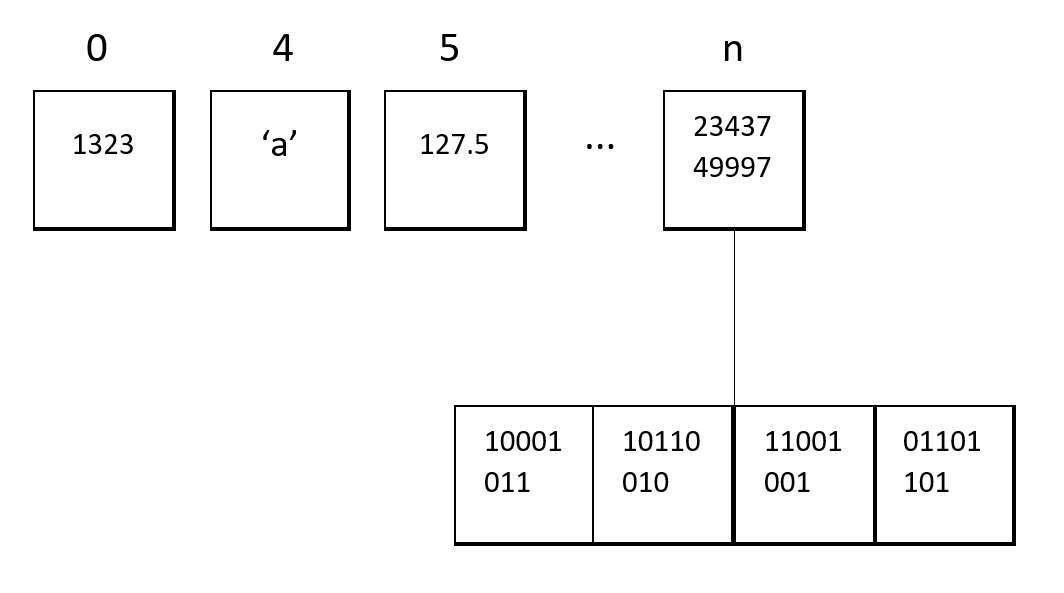
\includegraphics[scale=0.4]{Allocation.PNG}
		\caption{Memory Allocation of various data types}
		
	\end{figure}
	In Figure 1.1, the integer '1323' has taken 4 cubby holes or blocks sequentially from address '0' to '3'. Since a character is of 1 byte, character 'a' has taken only one cubby hole of address '4'.  The integer '234749997' has taken 4 cubby holes. Each cubby hole is of 8 bits or 1 byte. Therefore the binary representation of the integer is stored sequentially in the cubby holes. 
\newpage
\subsection{Conditional statements}
Conditional statements are used to make decisions based on a given condition.\\
\begin{figure}[H]
	\centering
	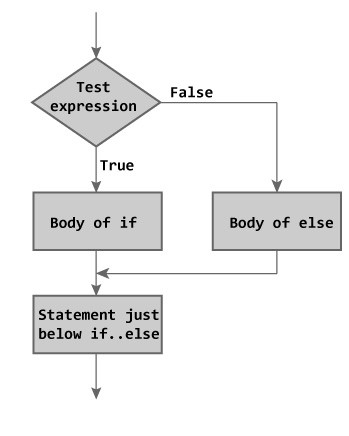
\includegraphics[scale=0.75]{if-else.jpg}
	\caption{Flowchart for if-else conditionals}
\end{figure}
~\\
\paragraph{Comparison operators with truth value}
Conditional statements works on the basis of the truth value of the expressions used.
There are multiple comparison operators which returns a truth value in boolean and are listed below. \\
\begin{table}[ht]
	\centering
	\begin{tabular}{|c|c|c|}
		\hline
		\thead{Operator} & \thead{Description} & \thead{Usage Example}\\
		\hline
		$==$ & equal to & \makecell{$1==1 \rightarrow$ true\\ 't' $==$ 'p' $\rightarrow$ false} \\
		\hline
		$!=$ & not equal to & \makecell{$5 != 5 \rightarrow$ false \\ $4.6 != 6.7 \rightarrow$ true }\\
		\hline
		$<$ & less than & \makecell{$5<4 \rightarrow$ false \\ 'a' $<$ 'b' $\rightarrow$ true ( using ASCII value)}\\
		\hline
		$<=$ & less than or equal to & \makecell{$4.5 <= 4.5 \rightarrow$ true \\ $3 <= 5.7 \rightarrow$ true }\\
		\hline
		$>=$& greater than or equal to & \makecell{'b' $>=$ 'b' $\rightarrow$ true \\ 
			true $>=$ false $\rightarrow$ true} \\
		\hline
		
	\end{tabular}
	\caption{Comparison operators}
	\label{tab:ComparisonOperators}
	
\end{table}
\begin{remark}
	Do not get confused between the assignment operator and equal to operator when using in an if conditional statement
\end{remark}
\newpage
The example below shows an example usage of if conditionals and comparison operators.
\begin{example}
	
	\begin{lstlisting}[title={Using if condition to check if number is divisible by 2},captionpos=b]
	#include <iostream>
	using namespace std;
	int main()
	{
	int num; //variable to store input
	cout<<"Enter number: "<<endl; //To show prompt
	cin>>num; //Taking and storing input value
	if(num % 2 == 0) //"a%b" to check the remainder when 'a' is  divided by 'b'
	{
	cout<<"Number is divisible by 2"<<endl;
	}
	else
	{
	cout<<"Number is not divisible by 2"<<endl;
	}
	return 0;
	}
	\end{lstlisting}
\end{example}
\subsection{Loops}
Loop is a sequence of instructions being repeated until a specific condition or target is reached. ~\\ ~\\
There are three types of loops in C++: \\
\paragraph{While loop}
A while loop statement repeatedly executes a target statement as long as a given condition is true. ~\\
The syntax of a while loop loop in C++ is:
\begin{lstlisting}
while (testExpression) 
{
	statement(s);
}
\end{lstlisting}
where, \textbf{testExpression} is checked on each entry of the while loop.
~\\ \\
Here is the flow of control in a while loop: \\
\begin{itemize}
\item The while loop evaluates the \textbf{test expression}.
If the \textbf{test expression} is true, codes inside the body of while loop is evaluated.
\item Then, the \textbf{test expression} is evaluated again. This process goes on until the \textbf{test expression} is false.
\item When the \textbf{test expression} is false, while loop is terminated.
\end{itemize}
\begin{figure}[H]
	\centering
	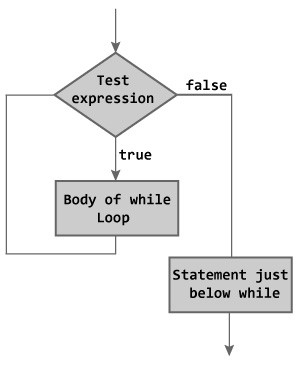
\includegraphics[scale=0.75]{while-loop.jpg}
	\caption{Flowchart of while loop}
\end{figure}
\begin{example}
	\begin{lstlisting}[title={Using While loop to increment an integer 5 times}, captionpos=b]
#include <iostream>
int main()
{
	int num = 1; //variable to be incremented
	int count = 0; //to keep track of number of iterations
	while(count < 5)
	{
		num = num + 1; //or num++ can also be used to increment
		count++;
	}
	return 0;
}
\end{lstlisting}
\end{example}
\paragraph{Do-while loop}
The syntax of do..while loop is:
\begin{lstlisting}
do {
	// codes;
}
while (testExpression);
\end{lstlisting}
Here is the flow of control in a while loop:
\begin{itemize}
\item The codes inside the body of loop is executed at least once. Then, only the \textbf{test expression} is checked.
\item If the \textbf{test expression} is true, the body of loop is executed. This process continues until the \textbf{test expression} becomes false.
\item When the \textbf{test expression} is false, do...while loop is terminated.
\end{itemize}
\begin{figure}[H]
	\centering
	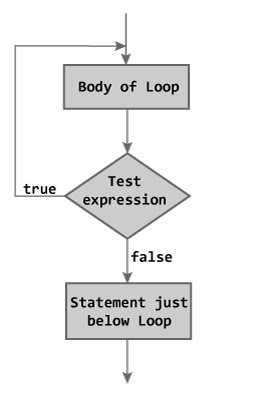
\includegraphics[scale=0.75]{dowhile-loop.jpg}
	\caption{Flowchart of do-while loop}
\end{figure}
\begin{example}
	\begin{lstlisting}[title={Using While loop to increment an integer 5 times}, captionpos=b]
#include <iostream>
int main()
{
	int num = 1; //variable to be incremented
	int count = 0; //to keep track of number of iterations
	do
	{
		num = num + 1; //or num++ can also be used to increment
		count++;
	}
	while(count<5)
	return 0;
}
\end{lstlisting}
\end{example}
\paragraph{For loop}
A for loop allows you to efficiently write a loop that needs to execute a specific number of times. ~\\
The syntax of a for loop in C++ is:
\begin{lstlisting}
for(initializationStatement; testExpression; updateStatement) 
{
	statement(s); 
}
\end{lstlisting}
Here is the flow of control in a for loop:
\begin{itemize}
\item The \textbf{initialization statement} is executed only once at the beginning.
\item Then, the \textbf{test expression} is evaluated.
If the \textbf{test expression} is false, for loop is terminated. But if the \textbf{test expression} is true, codes inside body of for loop is executed and \textbf{update statement} is executed.
\item Again, the \textbf{test expression} is evaluated and this process repeats until the \textbf{test expression} is false.
\end{itemize}
\begin{figure}[H]
	\centering
	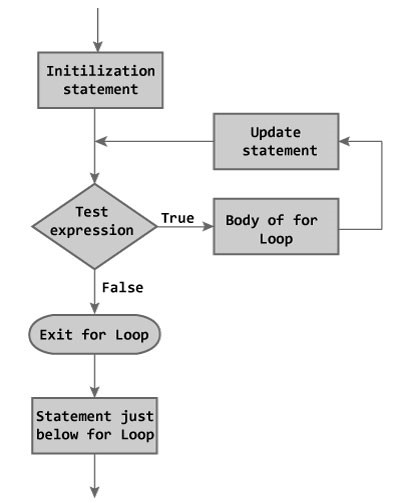
\includegraphics[scale=0.75]{for-loop.jpg}
	\caption{Flowchart of for loop}
\end{figure}
\begin{example}
	\begin{lstlisting}[title={Using For loop to increment an integer 5 times}, captionpos=b]
#include <iostream>
int main()
{
	int num = 1; //variable to be incremented
	for(int i = 0; i < 5; i++)
	{
		num = num + 1; //or num++ can also be used to increment
	}
	return 0;
}
\end{lstlisting}
\end{example}

\begin{example}
\begin{lstlisting}[title={Using While loop to increment an integer 5 times}, captionpos=b]
#include <iostream>
int main()
{
	int num = 1; //variable to be incremented
	int count = 0; //to keep track of number of iterations
	while(count < 5)
	{
		num = num + 1; //or num++ can also be used to increment
		count++;
	}
	return 0;
}
\end{lstlisting}
\end{example}
\newpage

\newpage
\subsection{Functions}
A function is a group of statements that together perform a task. Every C++ program has at least one function, which is main(), and all the most trivial programs can define additional functions.\\ ~\\ 
You can divide up your code into separate functions. How you divide up your code among different functions is up to you, but logically the division usually is such that each function performs a specific task. ~\\ ~\\
A function declaration tells the compiler about a function's name, return type, and parameters. A function definition provides the actual body of the function.
\paragraph{Defining a Function}
The general form of a C++ function definition is as follows:
\begin{lstlisting}
return_type function_name( parameter1, parameter2, parameter3,... ) 
{
	body of the function
}
\end{lstlisting} ~\\ ~\\
A C++ function definition consists of a function header and a function body. Here are all the parts of a function: ~\\
\begin{itemize}
\item \textbf{Return Type} - A function may return a value. The return\textunderscore type is the data type of the value the function returns. Some functions perform the desired operations without returning a value. In this case, the return\textunderscore type is the keyword void. \\
\item \textbf{Function Name} - This is the actual name of the function. The function name and the parameter list together constitute the function signature.\\
\item \textbf{Parameters} - A parameter is like a placeholder. When a function is invoked, you pass a value to the parameter. This value is referred to as actual parameter or argument. The parameter list refers to the type, order, and number of the parameters of a function. Parameters are optional; that is, a function may contain no parameters.\\
\item \textbf{Function Body} - The function body contains a collection of statements that define what the function does. ~\\
\end{itemize}

\paragraph{Declaring a function}
A function declaration tells the compiler about a function name and how to call the function. The actual body of the function can be defined separately.\\
\begin{lstlisting}
return_type function_name( parameter list );
\end{lstlisting}
\newpage
\paragraph{Calling a function}
While creating a C++ function, you give a definition of what the function has to do. To use a function, you will have to call or invoke that function. \\ ~\\
When a program calls a function, program control is transferred to the called function. A called function performs defined task and when it’s return statement is executed or when its function-ending closing brace is reached, it returns program control back to the main program. \\ ~\\
To call a function, you simply need to pass the required parameters along with function name, and if function returns a value, then you can store returned value.
\begin{example}
	\begin{lstlisting}[title={Declaration, definition amd calling of a max function},captionpos=b]
#include <iostream>
using namespace std;
	
// function declaration
int max(int num1, int num2);
	
int main () 
{
	// local variable declaration:
	int a = 100;
	int b = 200;
	int ret;
	
	// calling a function to get max value.
	ret = max(a, b);
	cout << "Max value is : " << ret << endl;
	
	return 0;
}
	
// function returning the max between two numbers
int max(int num1, int num2) 
{
	// local variable declaration
	int result;
	
	if (num1 > num2)
	result = num1;
	else
	result = num2;
	
	return result; 
}
	\end{lstlisting}
\end{example}
\newpage
\section{Problems}\index{Problems}
	\begin{problem}
		
		A certain grade of steel is graded according to the following conditions: ~\\
		\begin{itemize}
			\setlength\itemsep{1em}
			 \item Hardness must be greater than 50
			 \item Carbon content must be less than 0.7 \item Tensile strength must be greater than 5600
		\end{itemize}
		~\\ The grades are as follows: ~\\
		  \begin{itemize}
		  	\setlength\itemsep{1em}
		  \item Grade is 10 if all three conditions are met \item Grade is 9 if conditions (i) and (ii) are met
		  \item Grade is 8 if conditions (ii) and (iii) are met 
		  \item Grade is 7 if conditions (i) and (iii) are met
		  \item Grade is 6 if only one condition is met
		  \item Grade is 5 if none of the conditions are met
	\end{itemize}
		~\\Write a program, which will require the user to give values of hardness, carbon content and tensile strength of the steel under consideration and output the grade of the steel.
		\paragraph{Instructions}
		\begin{itemize}
			\item Use if-else conditional statements 
		\end{itemize}
	\end{problem}
~\\
\newpage
	\begin{problem}
		Two frogs named 'FrogPrime' and 'Frogatron' are in a well of depth 1000 feet. They decide to race each other to the top to see who is the winner.~\\ ~\\
		Both frogs can jump 4 feet at a time but slide down 1 foot every time, thus making the total distance covered to be 3 feet. ~\\ \\
		FrogPrime has a 2 \% chance to get an adrenaline rush and jump 5 feet.
		Frogatron has special claws that have a 2\% chance to grab on to a wall, thus it does not slide down 1 foot if the claws connect ~\\ \\
		The frogs will keep on jumping till one of them clears the well and is declared a winner. ~\\ \\
		Your program should simulate this behavior. It should find out the winner and report it. It should also report if there is a tie. ~\\ \\
		It should also display the progress of the frogs at every 50th jump.~\\ \\
		It should also display the total number of jumps once the competition is over. ~\\ \\
		The output should be similar to this:\\ \\
		\begin{center}
		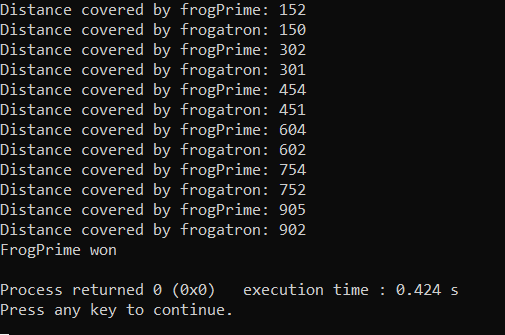
\includegraphics[scale=0.75]{Problem1_2.png}
		\end{center}
	\paragraph{Instructions}
	\begin{itemize}
		\item You can use random number generation to simulate chances. Find out yourself about using random number generation and ranges.
		\item Think in terms of loops and if-else conditionals
	\end{itemize}	
	
	\end{problem} ~\\ 
\begin{problem}
	Write a function IsPrime(int n) to test whether a parameter is prime. Apply the function in a program which prints all the prime numbers up to 100.
	\paragraph{Instructions}
	\begin{itemize}
		\item Use modulo operator to check divisibility
		\item You can use bool to keep check if a number is prime
		\item Break the question in parts and work on the function first
	\end{itemize}
\end{problem}
~\\
\begin{problem}
	Write a function Fibonacci(int n) which calculates the nth Fibonacci number. Write a main program that uses this function and the function from Problem 1.3 to print out the first 5 Fibonacci numbers that are also primes.
	\paragraph{Instructions}
	\begin{itemize}
		\item Think in terms of loops and an extensive use of variables to keep track of the needed terms in every iteration
	\end{itemize}
\end{problem}
\newpage
\section{Feedback}\index{Feedback}
\textbf{Please write the things you've learned from this lab and suggestions to make it more better and easy to learn.}

\chapter{Stacks}\index{Lab5: Stacks}
\section{Objective}\index{Objective}
In this lab, we'll learn about a data structure, called Stack. We'll learn about its implementation, operations and uses.
\section{Description}\index{Description}
Stack is a linear data structure which follows a particular order in which the operations are performed. The order may be LIFO (Last In First Out) or FILO (First In Last Out).\\ ~\\
Mainly the following three basic operations are performed in the stack:
\begin{itemize}
\item \textbf{Push}: Adds an item in the stack. If the stack is full, then it is said to be an Overflow condition.
\item \textbf{Pop}: Removes an item from the stack. The items are popped in the reversed order in which they are pushed. If the stack is empty, then it is said to be an Underflow condition.
\item \textbf{Peek or Top}: Returns top element of stack.
\item \textbf{isEmpty}: Returns true if stack is empty, else false.
\end{itemize}
\begin{figure}[H]
	\centering
	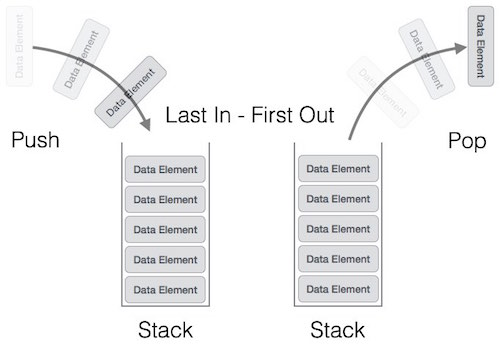
\includegraphics[scale=0.3]{stack.jpg}There are many real life examples of stack. Consider the simple example of plates stacked over one another in canteen. The plate which is at the top is the first one to be removed, i.e. the plate which has been placed at the bottommost position remains in the stack for the longest period of time. So, it can be simply seen to follow LIFO/FILO order.
	\caption{Representation of stack}
\end{figure}
\newpage
\subsection{Real-life example of stack}


\subsection{Time Complexities of operations on stack}
push(), pop(), isEmpty() and peek() all take O(1) time. We do not run any loop in any of these operations.

\subsection{Applications of stack}
There are many possible applications of stack. Some are listed below:
\begin{itemize}
	\item Balancing of symbols
	\item Infix to Postfix /Prefix conversion
	\item Redo-undo features at many places like editors, photoshop.
	\item Forward and backward feature in web browsers
	\item Used in many algorithms like Tower of Hanoi, tree traversals, stock span problem, histogram problem.
	\item Other applications can be Backtracking, Knight tour problem, rat in a maze, N queen problem and sudoku solver
\end{itemize}
\subsection{Implementation}\index{Implementation}
We will be implementing a linked list based stack. In a linked list based stack, we have nodes linked to each other.
Each node stores a data and a link to the node next to it.
\begin{figure}[H]
	\centering
	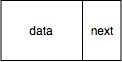
\includegraphics{node.jpg}
	\caption{Representation of node}
\end{figure}
\paragraph{Implementing Node}
To implement node, we will be making a struct to hold data and the link. In this implementation we are making a node to store integer type data. However, it can be implemented to store any data type or object.
\begin{lstlisting}
struct Node
{
	int data; \\To store data
	Node* next; \\To store the address or link to the next node
};
\end{lstlisting}
\newpage
\paragraph{Initializing the Stack}
As a stack consists of many nodes, we should have many nodes inside our stack class, but we will have only one node, "head", which will act as a reference node and allows us to iterate through all the nodes till the end of the stack.

\begin{lstlisting}
class Stack
{
	private:
		Node* head;
		
	public:
		Stack()
		{
			head = NULL;
		}
};		

\end{lstlisting}
Our stack now consists of a Node pointer which will hold the address of the head (i.e the top element) of the stack. To initialize, it is set to \textbf{NULL}, as the stack is empty.
\begin{figure}[H]
	\centering
	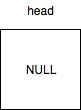
\includegraphics{head.jpg}
	\caption{Stack's head pointer}
\end{figure}

\paragraph{Implementing Push() operation}
Inside the class of Stack, we will declare and define a function "Push(int val)" in public.
\begin{lstlisting}
void Push(int val)
{
	if (head == NULL)
	{
		head = new Node;
		head->data = val;
		head->next = NULL;
	}
	else
	{
		Node* temp = head;
		head = new Node;
		head->data = val;
		head->next = temp;
	}
}
\end{lstlisting}
\newpage
\begin{example}
Let's visualize an example Push() operation\\
\begin{lstlisting}
Stack stack;
stack.Push(5);
\end{lstlisting}
Since the stack is empty and head is set to NULL. Body of 'if' will be executed.\\
It first creates a new node\\
\begin{figure}[H]
	\centering
	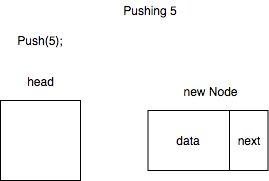
\includegraphics[scale=0.5]{push(1).jpeg}
	\caption{Creating new node for Push(5)}
\end{figure}
~\\
Then it sets head pointer to the new node.
\begin{figure}[H]
	\centering
	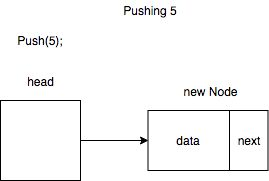
\includegraphics[scale=0.5]{push(2).jpeg}
	\caption{Setting head pointer}
\end{figure}
~\\
Then it sets the data and next pointer of new node.
\begin{figure}[H]
	\centering
	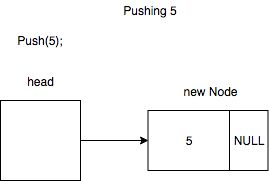
\includegraphics[scale=0.5]{push(3).jpeg}
	\caption{Setting data and next pointer}
\end{figure}
\end{example}
\newpage
Since, head is not \textbf{NULL}, Push operation will now execute body of 'else'. Let's see an example
\begin{example}
\begin{lstlisting}
stack.Push(3);
\end{lstlisting}
It will first create a temporary node pointer, temp.
\begin{figure}[H]
	\centering
	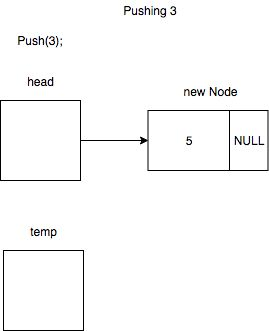
\includegraphics[scale=0.5]{push(4).jpeg}
	\caption{Creating temp pointer}
\end{figure} ~\\
Then it sets the temp to the node where head is pointing
\begin{figure}[H]
	\centering
	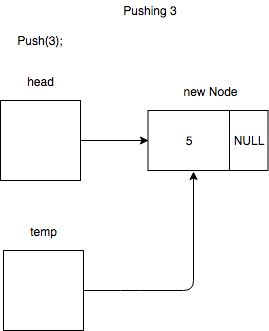
\includegraphics[scale=0.5]{push(5).jpg}
	\caption{Setting temp node}
\end{figure}
It now creates a new node and sets head to the newly created node.
\begin{figure}[H]
	\centering
	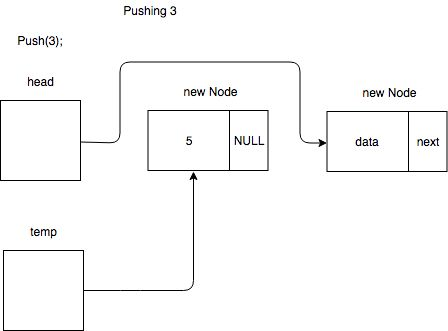
\includegraphics[scale=0.5]{push(6).jpeg}
	\caption{Setting head to the new node}
\end{figure}
It sets the newly created node's next pointer to the node being pointed by temp.
\begin{figure}[H]
	\centering
	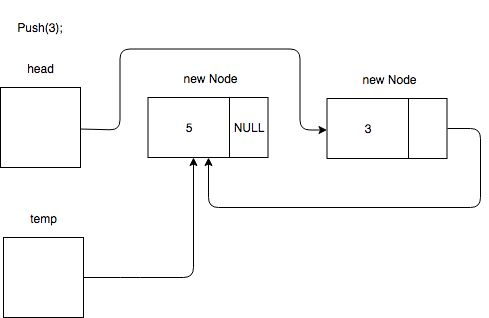
\includegraphics[scale=0.5]{push(7).jpg}
	\caption{Setting next pointer}
\end{figure}
The temp gets destroyed since it was a local variable of the function and 3 is added succesfully.
\textsc{\begin{figure}[H]
	\centering
	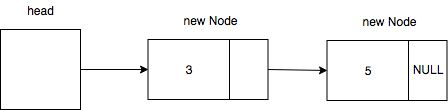
\includegraphics[scale=0.5]{push(8).jpeg}
	\caption{Succesful Push(3) operation}
\end{figure}}
\end{example}
\newpage
\paragraph{Implementing Pop() Operation}
Inside the class of Stack, we will declare and define a function "Pop()" in public.
\begin{lstlisting}
int Pop()
{
	int val = -1;
	if(head != NULL)
	{
		Node* temp = head;
		head = head->next;
		val = temp->data;
		delete temp;
		temp = NULL;
	}
	return val;
}
\end{lstlisting}
Let's visualize an example of Pop() operation
\begin{example}
	\begin{lstlisting}
stack.Pop();
	\end{lstlisting}

This is the stack on which pop() will be called.
\begin{figure}[H]
	\centering
	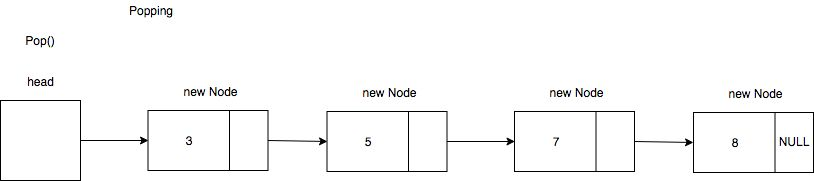
\includegraphics[scale=0.5]{pop(1).jpeg}
	\caption{Stack before pop()}
\end{figure} ~\\
After checking the head pointer if it is not NULL, it creates a temp pointer and stores the address of node pointed by head in it.
\begin{figure}[H]
	\centering
	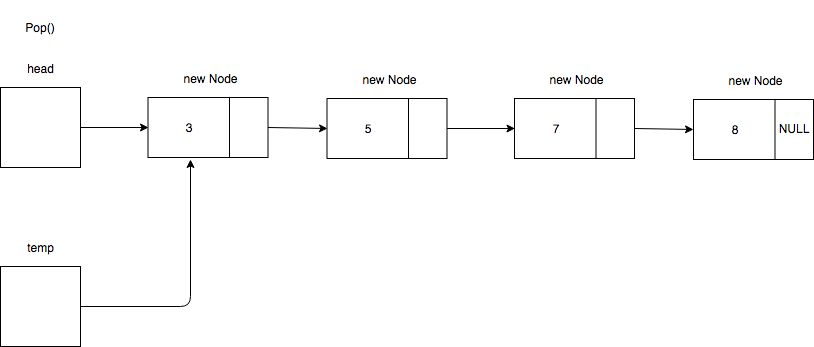
\includegraphics[scale=0.5]{pop(2).jpeg}
	\caption{Creating temp pointer}
\end{figure} ~\\
It updates the head pointer to the node next to head
\begin{figure}[H]
	\centering
	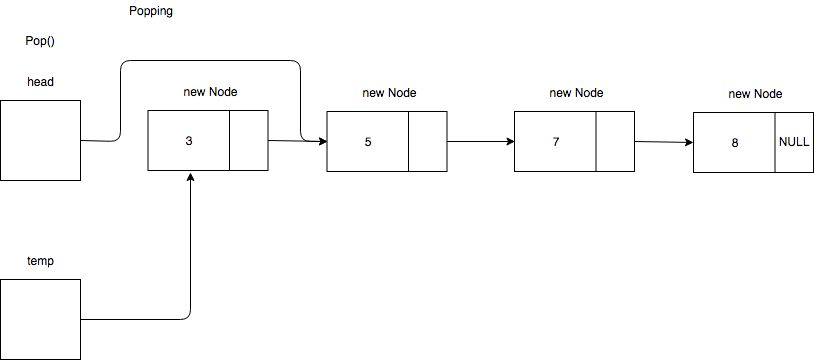
\includegraphics[scale=0.5]{pop(3).jpeg}
	\caption{Updating head pointer}
\end{figure} ~\\
It now deletes the node pointed by temp.
\begin{figure}[H]
	\centering
	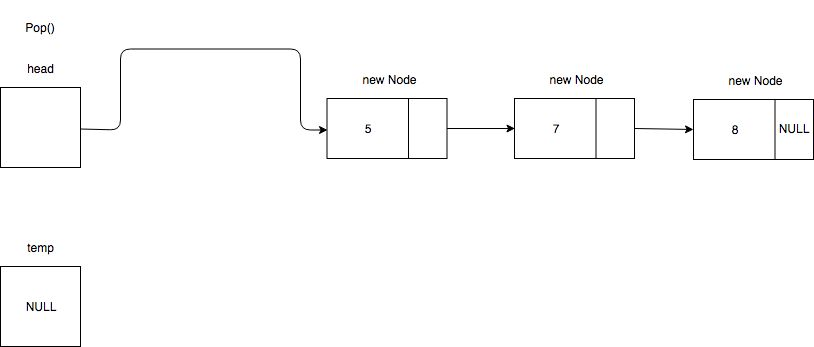
\includegraphics[scale=0.5]{pop(4).jpeg}
	\caption{Deleting the node pointed by temp}
\end{figure} ~\\
The temp pointer then gets destroyed and stack is updated successfully.
\begin{figure}[H]
	\centering
	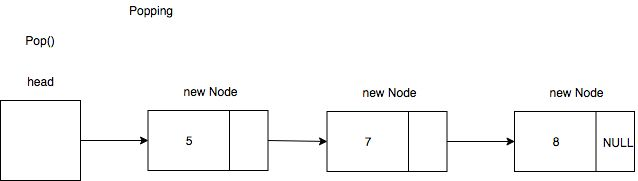
\includegraphics[scale=0.5]{pop(5).jpeg}
	\caption{Succesful pop() operation}
\end{figure}
\end{example} ~\\
\paragraph{Implementing Show() function}
The Show()  function allows to output all the values in the stack. \\
Inside the class of Stack, we will declare and define a function "void Show()" in public.
\begin{lstlisting}
void Show()
	Node* temp = head;
	while(temp!=NULL)
	{
		std::cout<<temp->data<<std::endl;
		temp = temp->next;
	}
\end{lstlisting}

Let's visualize an example of Show() operation
\begin{example}
	\begin{lstlisting}
	stack.Show();
	\end{lstlisting}
Creating the temp pointer and points it to the node pointed by head.
\begin{figure}[H]
	\centering
	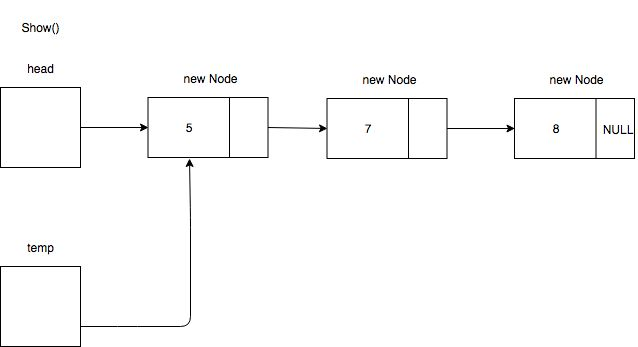
\includegraphics[scale=0.5]{show(1).jpeg}
	\caption{Creating temp pointer}
\end{figure} ~\\
Now it outputs the vaue stored in the node pointed by temp.
\begin{figure}[H]
	\centering
	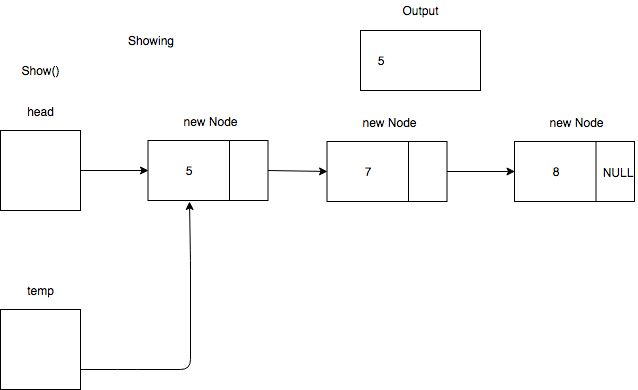
\includegraphics[scale=0.5]{show(2).jpeg}
	\caption{Outputting first value}
\end{figure} ~\\
It updates the temp pointer and moves to the next node. Then it outputs the value of the node pointed by temp.
\begin{figure}[H]
	\centering
	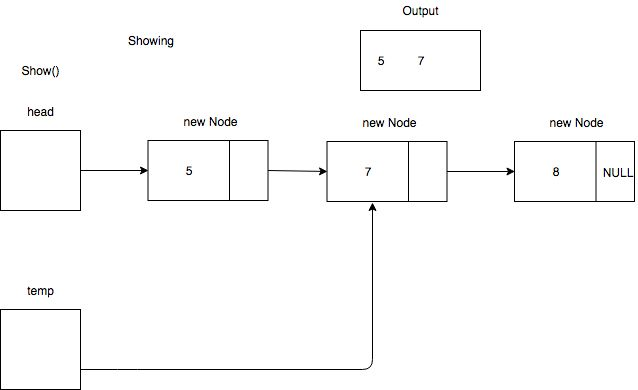
\includegraphics[scale=0.5]{show(3).jpeg}
	\caption{Updating temp pointer and outputting value}
\end{figure} ~\\
It repeats the updating of temp pointer and outputs the value
\begin{figure}[H]
	\centering
	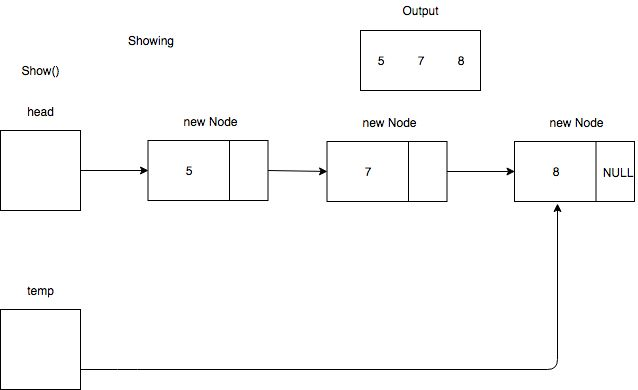
\includegraphics[scale=0.5]{show(4).jpeg}
	\caption{Updating the temp pointer to the third node and outputs the value}
\end{figure} ~\\
The loop gets stopped now because the temp is now set to NULL.
\begin{figure}[H]
	\centering
	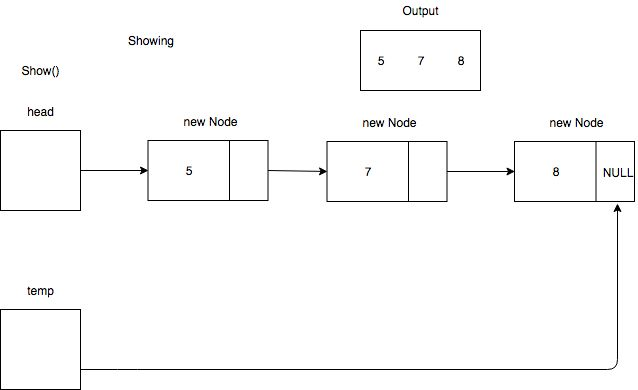
\includegraphics[scale=0.5]{show(5).jpeg}
	\caption{Updating the temp pointer to the third node and outputs the value}
\end{figure}
\end{example}
 \section{Problems}\index{Problems}
 \begin{problem}
 	Implement the isEmpty() function in your Stack class. The function should return true if the stack is empty and return false if not.
 	\paragraph{Instructions}
 	\begin{itemize}
 		\item Think about the value stored in head pointer when the stack is Empty
 	\end{itemize}
 \end{problem}
~\\
\begin{problem}
	Implement the  functions Top() and Bottom() in your Stack class. The Top() function should return the top element of the stack. The Bottom() function should return the element on the bottom of the stack.
	\paragraph{Instructions}
		\begin{itemize}
			\item Top() function is easy to implement after doing the problem above. Use head pointer to implement this function
			\item For Bottom() function, think how to iterate over the stack till the bottom using only head pointer and a temporary pointer.
		\end{itemize}
\end{problem}
\newpage


\section{Feedback}\index{Feedback}
\textbf{Please write the things you've learned from this lab and suggestions to make it more better and easy to learn.}

\chapter{Double-linked list}
\section{Objective}\index{Objective}
In this lab, we'll learn about a data structure, called Double linked list. We'll learn about its implementation, operations and uses.
\section{Description}\index{Description}
Double linked list is a sequence of elements in which every element has links to its previous element and next element in the sequence.
It has the same operations as the single-linked list, but the opertions takes less time as there ire shorter traversals using links to both next and previous element. We'll see it in the examples below.
 
\subsection{Real-life examples of Double linked list}
There are many real life examples of stack. Consider the simple example of a music player. The music player allows skipping to both next and previous song in the playlist. Moreover, it allows to traverse through the list to find a song using both next and previous buttons.

\subsection{Time Complexities of Double linked list}
Append(data) - O(1) time \\
Add(i, data) - O(min(i, n - i))\\
Remove(i) - O(min(i, n - i))\\ 
Where i is the index and n is the size of the list.\\ \\
For add and remove, we have to find the node at the index where a node is getting added or removed. Finding the node with a particular index in a DLList is easy; we can either start at the head of the list and work forward ,or start at the tail of the list and work backward. This allows us to reach the ith node in O(min(i,n - i)) time.
 
\subsection{Applications of Double linked list}
There are many possible applications of stack. Some are listed below:
\begin{itemize}
	\item The browser cache which allows you to hit the BACK buttons (a linked list of URLs).
	\item Applications that have a Most Recently Used (MRU) list (a linked list of file names).
	\item A stack, hash table, and binary tree can be implemented using a doubly linked list. 
	\item Undo functionality in Photoshop or Word (a linked list of state).
\end{itemize}

\section{Implementation}
We will be implementing a double linked list. In double linked list, we have nodes linked to each other.
Each node stores a data and links to the node next to and previous to it.
\begin{figure}[H]
	\centering
	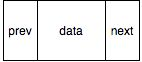
\includegraphics{DLNode.jpeg}
	\caption{Representation of node}
\end{figure}
\paragraph{Implementing Node}
To implement node, we will be making a struct to hold data and the links to store next and previous node . In this implementation we are making a node to store integer type data. However, it can be implemented to store any data type or object.
\begin{lstlisting}
struct Node
{
	int data;
	Node* next;
	Node* prev;
	Node()
	{
		next = NULL;
		prev = NULL;
	}
};
\end{lstlisting}
\paragraph{Initializing the Double linked list}
As a Double linked consists of many nodes, we should have many nodes inside our DLList class, but we will have only two nodes, "head" and "tail", which will act as reference nodes and allows us to iterate through all the nodes in the DLList. Moreover, we will include an integer "Size" to keep track of the size of the list.
\begin{lstlisting}
class DLList
{
	private:
		int Size;
		Node* head;
		Node* tail;
	public:
		DLList()
		{
			head = NULL;
			tail = NULL:
		}
}
\end{lstlisting}
Our stack now consists of Node pointers which will hold the addresses of the head and the tail. To initialize, both are set to \textbf{NULL}, as the list is empty.
\begin{figure}[H]
	\centering
	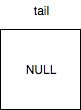
\includegraphics{DLList1.jpeg}
	\caption{DLList head pointer}
\end{figure}
\begin{figure}[H]
	\centering
	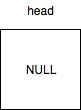
\includegraphics{DLList2.jpeg}
	\caption{DLList tail pointer}
\end{figure}
\paragraph{Implementing Append operation}
Inside the class of DLList, we will declare and define a function "Append(int data)" in public.
\begin{lstlisting}
void Append(int data)
{
	if (Size == 0)
	{
		head = tail = new Node();
		head->data = data;
	}
	else
	{
		tail->next = new Node();
		tail->next->prev = tail;
		tail = tail->next;
		tail->data = data;
	}
	Size++;
}

\end{lstlisting}
\begin{example}
	Let's visualize an example Append() operation\\
	\begin{lstlisting}
	DLList lst;
	lst.Append(6);
	\end{lstlisting}
	Since the DLList is empty and head is set to NULL. Body of 'if' will be executed.\\
	It first creates a new node and sets head and tail to it.\\
	\begin{figure}[H]
		\centering
		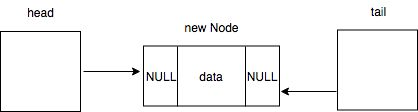
\includegraphics[scale=0.5]{DLList3.jpeg}
		\caption{Creating new node}
	\end{figure}
	~\\
	Then it sets its data to the data passed.
	\begin{figure}[H]
		\centering
		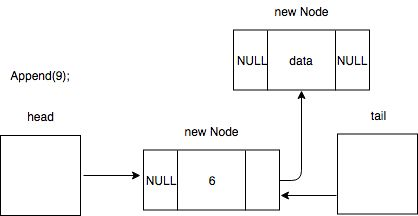
\includegraphics[scale=0.5]{DLList4.jpeg}
		\caption{Setting data}
	\end{figure}
\end{example}
Since, Size is not '0', Append operation will now execute body of 'else'. Let's see an example
\begin{example}
	\begin{lstlisting}
	lst.append(9);
	\end{lstlisting}
	It will first create a new node and sets tail's next to it.
	\begin{figure}[H]
		\centering
		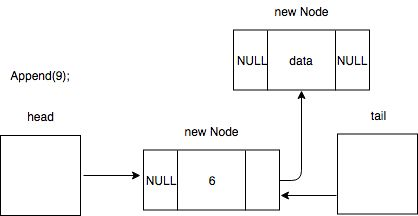
\includegraphics[scale=0.5]{DLList4.jpeg}
		\caption{Creating new node}
	\end{figure} ~\\
	Then it sets the new node's prev to the tail
	\begin{figure}[H]
		\centering
		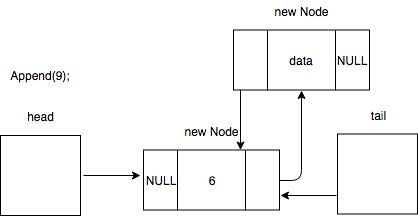
\includegraphics[scale=0.5]{DLList5.jpeg}
		\caption{Setting new node's pointer}
	\end{figure}
	It now updates the tail and sets data.
	\begin{figure}[H]
		\centering
		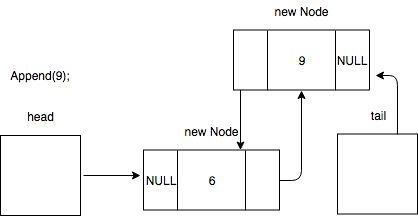
\includegraphics[scale=0.5]{DLList6.jpeg}
		\caption{Updating tail and data}
	\end{figure}
		'9' is added succesfully.
	{\begin{figure}[H]
			\centering
			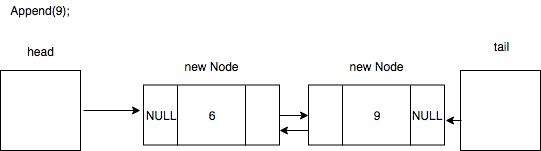
\includegraphics[scale=0.5]{DLList7.jpeg}
			\caption{Succesful Append(9) operation}
	\end{figure}}
\end{example}
\paragraph{Implementing Add operation}
Inside the class of DLList, we will declare and define a function "Append(int data)" in public.
\begin{lstlisting}
void Add(int i, int data)
{
	if(i >= 0 && i <= Size)
	{
		if (i == 0)
		{
			if (Size == 0)
			{
				head = tail = new Node();
				head->data = data;
			}
			else
			{
				head->prev = new Node;
				head->prev->next = head;
				head = head->prev;
				head->data = data;
			}
			
		}
		else if (i == Size)
		{
			tail->next = new Node();
			tail->next->prev = tail;
			tail = tail->next;
			tail->data = data;
		}
		else
		{
			Node* temp;
			if (i <= Size/2)
			{
				temp = head;
				for (int j = 0; j < i; j++)
				{
					temp=temp->next;
				}
			}	
			else
			{
				temp = tail;
				for (int j = 0; j < Size-i-1; j++)
				{
				temp = temp->prev;
				}
			}
		
			Node* newNode = new Node;
			newNode->data = data;
			newNode->prev = temp->prev;
			newNode->next = temp;
			temp->prev->next = newNode;
			temp->prev = newNode;
			
		}
		Size++;
	}
	else
	{
		cout << "Index is out of range" << endl;
	}
}

\end{lstlisting}
\begin{example}
	Let's visualize an example Add() operation\\
	\begin{lstlisting}
	DLList lst;
	lst.Add(0,6);
	\end{lstlisting}
	Since the DLList is empty, Body of 'if (i == 0) and if (Size == 0)' will be executed.\\
	It wll carry out the same operations carried out in Append function.\\
	It first creates a new node and sets head and tail to it.\\
	\begin{figure}[H]
		\centering
		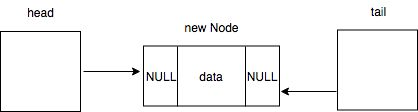
\includegraphics[scale=0.5]{DLList3.jpeg}
		\caption{Creating new node}
	\end{figure}
	~\\
	Then it sets its data to the data passed.
	\begin{figure}[H]
		\centering
		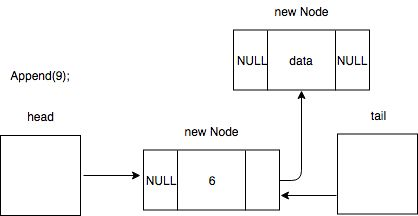
\includegraphics[scale=0.5]{DLList4.jpeg}
		\caption{Setting data}
	\end{figure}
\end{example}
If a number is added to the last, it will then also do the same tasks as append.\\

\begin{example}
	\begin{lstlisting}
	lst.Add(1,9);
	\end{lstlisting}
	Now size is not 0 and index is equal to the size.\\
	It will first create a new node and sets tail's next to it.
	\begin{figure}[H]
		\centering
		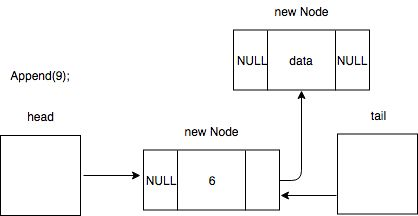
\includegraphics[scale=0.5]{DLList4.jpeg}
		\caption{Creating new node}
	\end{figure} ~\\
	Then it sets the new node's prev to the tail
	\begin{figure}[H]
		\centering
		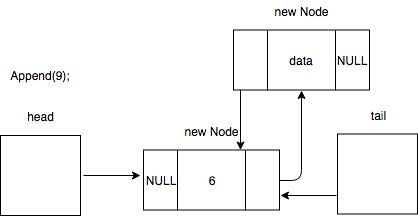
\includegraphics[scale=0.5]{DLList5.jpeg}
		\caption{Setting new node's pointer}
	\end{figure}
	It now updates the tail and sets data.
	\begin{figure}[H]
		\centering
		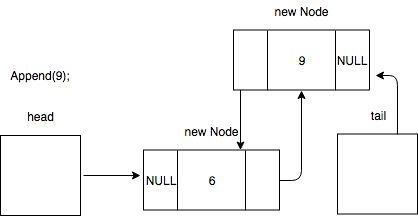
\includegraphics[scale=0.5]{DLList6.jpeg}
		\caption{Updating tail and data}
	\end{figure}
	'9' is added succesfully.
	{\begin{figure}[H]
			\centering
			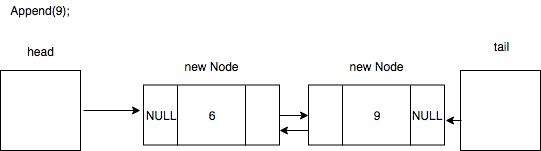
\includegraphics[scale=0.5]{DLList7.jpeg}
			\caption{Succesful Add(1,9) operation}
	\end{figure}}
\end{example}
\begin{example}
Let's look at an example, when index is neither 0 nor equal to the size.
Let's visualize an example Add() operation\\
\begin{lstlisting}
lst.Add(1,5);
\end{lstlisting}
Since i is less than half of the size, it will iterate from the head.\\
It will first create a temporary pointer and point it to head.
\begin{figure}[H]
	\centering
	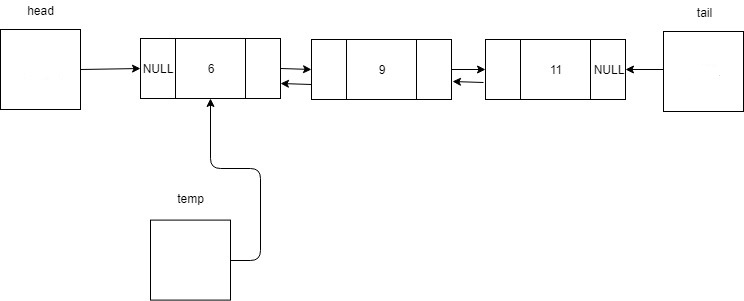
\includegraphics[scale=0.5]{DLAdd1.jpg}
	\caption{Creating a temporary pointer}
\end{figure} ~\\
It will iterate till it reaches the index where a new node is to be added.
\begin{figure}[H]
	\centering
	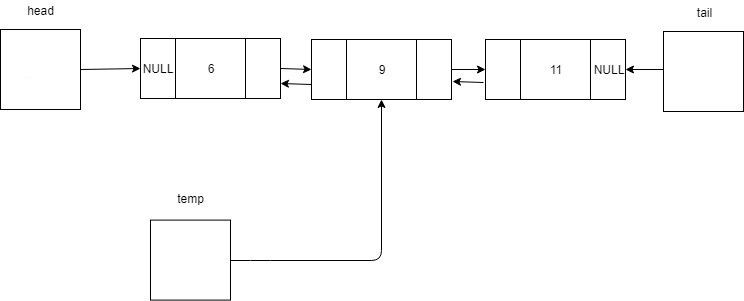
\includegraphics[scale=0.5]{DLAdd2.jpg}
	\caption{Iterating till it reaches the node}
\end{figure}
It will create a new Node.
\begin{figure}[H]
	\centering
	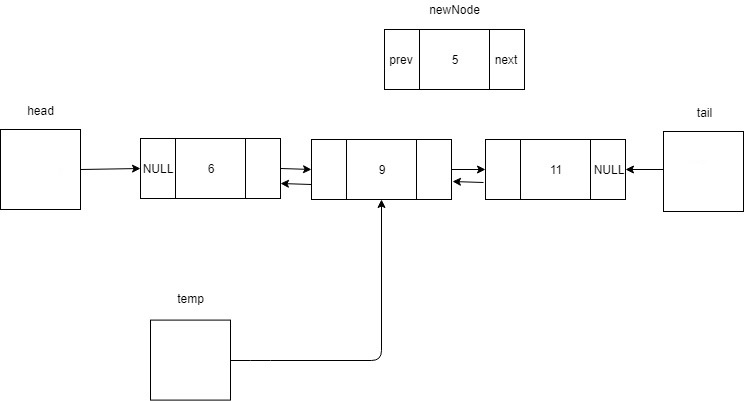
\includegraphics[scale=0.5]{DLAdd3.jpg}
	\caption{Creating new node}
\end{figure}
Points its 'prev' pointer to the temp's 'prev'.
\begin{figure}[H]
	\centering
	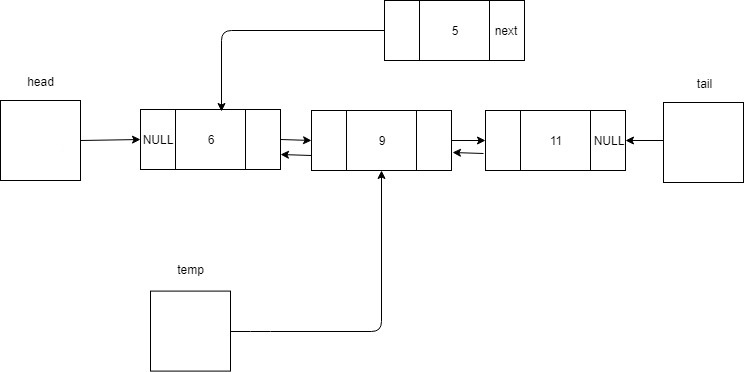
\includegraphics[scale=0.5]{DLAdd4.jpg}
	\caption{Setting node's prev pointer}
\end{figure}~\\
Points its 'next' pointer to temp.
\begin{figure}[H]
	\centering
	\includegraphics[scale=0.5]{DLAdd5.jpg}
	\caption{Setting node's next pointer}
\end{figure}
Point Node's prev's next pointer to itself.
\begin{figure}[H]
	\centering
	\includegraphics[scale=0.5]{DLAdd5(1).jpg}
	\caption{Setting the previous node's next pointer}
\end{figure}
And finally temp's prev to the new node.
\begin{figure}[H]
	\centering
	\includegraphics[scale=0.5]{DLAdd6.jpg}
	\caption{Succesful addition}
\end{figure}
\end{example}
\begin{example}
Now, let's see an example where index is greater than the half of the size of the list.\\
\begin{lstlisting}
lst.Add(2,13);
\end{lstlisting}
Since index is greater than the half of the size, it will start iteration from the last.\\
It will first create a temporary pointer and sets it to the tail.
\begin{figure}[H]
	\centering
	\includegraphics[scale=0.5]{DLAdd7.jpg}
	\caption{Creating a temporary pointer}
\end{figure}
It will iterate till it reaches the index where the new node has to be added
\begin{figure}[H]
	\centering
	\includegraphics[scale=0.5]{DLAdd8.jpg}
	\caption{Iterated till the index}
\end{figure}
Now it repeats the same process of setting pointers as it did above and adds the new node succesfully.
\begin{figure}[H]
	\centering
	\includegraphics[scale=0.5]{DLAdd10.jpg}
	\caption{Succesful Add(2,13) operation}
\end{figure}
\end{example}
Let's see an example when the size is not '0' and the node is to be added at index '0'.
\begin{example}
	\begin{lstlisting}
	lst.Add(0,4);
	\end{lstlisting}
It will first create a new node and sets the prev's pointer, of the node pointed by head, to it.
\begin{figure}[H]
	\centering
	\includegraphics[scale=0.5]{DLAdd11.jpg}
	\caption{Creating new node and setting head's prev}
\end{figure}~\\
Then it sets new node's next to the next of node pointed by head.
\begin{figure}[H]
	\centering
	\includegraphics[scale=0.5]{DLAdd12.jpg}
	\caption{Setting node's next pointer}
\end{figure}~\\
Finally, head is set to the new node and the node is added succesfully.
\begin{figure}[H]
	\centering
	\includegraphics[scale=0.5]{DLAdd13.jpg}
	\caption{Updating head}
\end{figure}
\end{example}
\paragraph{Implementing Show() function}
The Show()  function allows to output all the values in the DLList. \\
Inside the class of DLList, we will declare and define a function "void Show()" in public.
\begin{lstlisting}
void Show()
{
	Node* temp = head;
	while(temp!=NULL)
	{
		std::cout<<temp->data<<std::endl;
		temp = temp->next;
	}
}
\end{lstlisting}~\\
Let's visualize an example of Show() operation
\begin{example}
	\begin{lstlisting}
lst.Show();
	\end{lstlisting}~\\
It creates a temp pointer and is pointed to the node pointed by head. It also outputs its value
\begin{figure}[H]
	\centering
	\includegraphics[scale=0.5]{DLShow1.jpg}
	\caption{Creating temp pointer and outputting first value}
\end{figure} ~\\
It updates the temp pointer and moves to the next node. Then it outputs the value of the node pointed by temp.
\begin{figure}[H]
	\centering
	\includegraphics[scale=0.5]{DLShow2.jpg}
	\caption{Outputting second value}
\end{figure} ~\\
And finally it moves to the last node, outputs its value and since it's next is equal to NULL, the loop is ended.
\begin{figure}[H]
	\centering
	\includegraphics[scale=0.5]{DLShow3.jpg}
	\caption{Outputting third value}
\end{figure} ~\\
\end{example}
\section{Problems}\index{Problems}
\begin{problem}
	Implement the Remove(int index) function in your DLList class. The function should remove the element from the given index and returns the removed element. The function should run in O(min(i, n - i)).
	\paragraph{Instructions}
	\begin{itemize}
		\item Think for all special cases such as, removal at zero index and removal at last index.
		\item Update pointers carefully.
		\item Try to take an idea from given Add() function for traversal.
	\end{itemize}
\end{problem}
~\\
\begin{problem}
	Implement the function Reverse() which reverses the list, without making a new list.
	\paragraph{Instructions}
	\begin{itemize}
		\item Traverse through the whole list and update its pointers accordingly
	\end{itemize}
\end{problem}
\newpage
\section{Feedback}\index{Feedback}
\textbf{Please write the things you've learned from this lab and suggestions to make it more better and easy to learn.}

\chapter{Abstract classes}
\section{Objective}
In this lab, we will learn about a type of class called abstract classes and its usage and implementation.
\section{Description}
\begin{figure}[H]
	\centering
	\includegraphics[scale=0.5]{UML.jpeg}
	\caption{UML representation of abstract class}
\end{figure} ~\\
Sometimes implementation of all function cannot be provided in a base class because we don’t know the implementation. Such a class is called \textbf{abstract class}. For example, let Shape be a base class. We cannot provide implementation of function draw() in Shape, but we know every derived class must have implementation of draw(). Similarly an Animal class doesn’t have implementation of move() (assuming that all animals move), but all animals must know how to move. We cannot create objects of abstract classes. For this, we need to have at least one pure virtual function in the class. \\
A \textbf{pure virtual function} (or abstract function) in C++ is a virtual function for which we don’t have implementation, we only declare it. A pure virtual function is declared by assigning 0 in declaration. It's done by the syntax showed below.
\begin{lstlisting}
// An abstract class
class Test
{   
	// Data members of class
	public:
	// Pure Virtual Function
	virtual void show() = 0;

	/* Other members */
};
\end{lstlisting} ~\\
Let's see an example in whch a pure virtual function is declared in the abstract class and then defined in the derived class.
\begin{example}
\begin{lstlisting}
class Base
{
	int x;
	public:
		virtual void func() = 0;
		int getX() 
		{
			return x; 
		}
};

// This class inherits from Base and implements func()
class Derived: public Base
{
	int y;
	public:
		void func()
		{
			cout << "func() called";
		}
};

int main()
{
	Derived d;
	d.func();
	return 0;
}
\end{lstlisting}
Now the abstract class has the attribute 'int x' and the function 'int GetX()'. This function will also be the part of derived class and is already defined in the base class. Now the function 'func()' is a pure virtual function which is defined in the base class and is implemented in the derived class. Now, if we create an instance of Derived class, we can access the functions 'GetX()' and 'func()'. The 'GetX()' will be called through the base class and 'func()' will be called through the derived class.
The program above will output:
\begin{figure}[H]
	\centering
	\includegraphics[scale=0.5]{Class.png}
	\caption{Output of implemented pure virtual function}
\end{figure}
\end{example}
The derived class can also become an abstract class if the pure virtual function declared in base class is not defined in the derived class.
\begin{example}
\begin{lstlisting}
class Base
{
	public:
	virtual void show() = 0;
};

class Derived : public Base { };

int main(void)
{
	Derived d;
	return 0;
}
\end{lstlisting}
\end{example}
\begin{corollary}[Interface vs Abstract classes]
An interface does not have implementation of any of its methods, it can be considered as a collection of method declarations. In C++, an interface can be simulated by making all methods as pure virtual. In Java, there is a separate keyword for interface.
\end{corollary}
\newpage
\section{Problems}
\begin{problem}
	Make an abstract class of Shape with pure virtual function to calculate area. It should also have the attributes for the position of the Shape. The derived classes should be Square, Circle, Trapezium and Rectangle. All derived classes should implement the pure virtual function defined in the base class. 
	\paragraph{Instructions}
	\begin{itemize}
		\item Make a struct for Position to have x and y coordinates.
		\item Define the attributes for dimensions according to the shape in derived classes
	\end{itemize}
\end{problem}
\begin{problem}
	Make a base class with a pure virtual function. Derive a class from it and declare another pure virtual function in the derived class. Then derive an other class from the first derived class and declare a pure virtual function in it too. And then lastly derive another class from the second derived class, and define all the pure virtual functions in it
\end{problem}
\newpage
\section{Feedback}\index{Feedback}
\textbf{Please write the things you've learned from this lab and suggestions to make it more better and easy to learn.}
%----------------------------------------------------------------------------------------
%	CHAPTER 2
%----------------------------------------------------------------------------------------



\chapter{In-text Elements}

\section{Theorems}\index{Theorems}

This is an example of theorems.

\subsection{Several equations}\index{Theorems!Several Equations}
This is a theorem consisting of several equations.

\begin{theorem}[Name of the theorem]
In $E=\mathbb{R}^n$ all norms are equivalent. It has the properties:
\begin{align}
& \big| ||\mathbf{x}|| - ||\mathbf{y}|| \big|\leq || \mathbf{x}- \mathbf{y}||\\
&  ||\sum_{i=1}^n\mathbf{x}_i||\leq \sum_{i=1}^n||\mathbf{x}_i||\quad\text{where $n$ is a finite integer}
\end{align}
\end{theorem}

\subsection{Single Line}\index{Theorems!Single Line}
This is a theorem consisting of just one line.

\begin{theorem}
A set $\mathcal{D}(G)$ in dense in $L^2(G)$, $|\cdot|_0$. 
\end{theorem}

%------------------------------------------------

\section{Definitions}\index{Definitions}

This is an example of a definition. A definition could be mathematical or it could define a concept.

\begin{definition}[Definition name]
Given a vector space $E$, a norm on $E$ is an application, denoted $||\cdot||$, $E$ in $\mathbb{R}^+=[0,+\infty[$ such that:
\begin{align}
& ||\mathbf{x}||=0\ \Rightarrow\ \mathbf{x}=\mathbf{0}\\
& ||\lambda \mathbf{x}||=|\lambda|\cdot ||\mathbf{x}||\\
& ||\mathbf{x}+\mathbf{y}||\leq ||\mathbf{x}||+||\mathbf{y}||
\end{align}
\end{definition}

%------------------------------------------------

\section{Notations}\index{Notations}

\begin{notation}
Given an open subset $G$ of $\mathbb{R}^n$, the set of functions $\varphi$ are:
\begin{enumerate}
\item Bounded support $G$;
\item Infinitely differentiable;
\end{enumerate}
a vector space is denoted by $\mathcal{D}(G)$. 
\end{notation}

%------------------------------------------------

\section{Remarks}\index{Remarks}

This is an example of a remark.

\begin{remark}
The concepts presented here are now in conventional employment in mathematics. Vector spaces are taken over the field $\mathbb{K}=\mathbb{R}$, however, established properties are easily extended to $\mathbb{K}=\mathbb{C}$.
\end{remark}

%------------------------------------------------

\section{Corollaries}\index{Corollaries}

This is an example of a corollary.

\begin{corollary}[Corollary name]
The concepts presented here are now in conventional employment in mathematics. Vector spaces are taken over the field $\mathbb{K}=\mathbb{R}$, however, established properties are easily extended to $\mathbb{K}=\mathbb{C}$.
\end{corollary}

%------------------------------------------------

\section{Propositions}\index{Propositions}

This is an example of propositions.

\subsection{Several equations}\index{Propositions!Several Equations}

\begin{proposition}[Proposition name]
It has the properties:
\begin{align}
& \big| ||\mathbf{x}|| - ||\mathbf{y}|| \big|\leq || \mathbf{x}- \mathbf{y}||\\
&  ||\sum_{i=1}^n\mathbf{x}_i||\leq \sum_{i=1}^n||\mathbf{x}_i||\quad\text{where $n$ is a finite integer}
\end{align}
\end{proposition}

\subsection{Single Line}\index{Propositions!Single Line}

\begin{proposition} 
Let $f,g\in L^2(G)$; if $\forall \varphi\in\mathcal{D}(G)$, $(f,\varphi)_0=(g,\varphi)_0$ then $f = g$. 
\end{proposition}

%------------------------------------------------

\section{Examples}\index{Examples}

This is an example of examples.

\subsection{Equation and Text}\index{Examples!Equation and Text}

\begin{example}
Let $G=\{x\in\mathbb{R}^2:|x|<3\}$ and denoted by: $x^0=(1,1)$; consider the function:
\begin{equation}
f(x)=\left\{\begin{aligned} & \mathrm{e}^{|x|} & & \text{si $|x-x^0|\leq 1/2$}\\
& 0 & & \text{si $|x-x^0|> 1/2$}\end{aligned}\right.
\end{equation}
The function $f$ has bounded support, we can take $A=\{x\in\mathbb{R}^2:|x-x^0|\leq 1/2+\epsilon\}$ for all $\epsilon\in\intoo{0}{5/2-\sqrt{2}}$.
\end{example}

\subsection{Paragraph of Text}\index{Examples!Paragraph of Text}

\begin{example}[Example name]
\lipsum[2]
\end{example}

%------------------------------------------------

\section{Exercises}\index{Exercises}

This is an example of an exercise.

\begin{exercise}
This is a good place to ask a question to test learning progress or further cement ideas into students' minds.
\end{exercise}

%------------------------------------------------

\section{Problems}\index{Problems}

\begin{problem}
What is the average airspeed velocity of an unladen swallow?
\end{problem}

%------------------------------------------------

\section{Vocabulary}\index{Vocabulary}

Define a word to improve a students' vocabulary.

\begin{vocabulary}[Word]
Definition of word.
\end{vocabulary}

%----------------------------------------------------------------------------------------
%	PART
%----------------------------------------------------------------------------------------

\part{Part Two}

%----------------------------------------------------------------------------------------
%	CHAPTER 3
%----------------------------------------------------------------------------------------

\chapterimage{chapter_head_1.pdf} % Chapter heading image

\chapter{Presenting Information}

\section{Table}\index{Table}

\begin{table}[h]
\centering
\begin{tabular}{l l l}
\toprule
\textbf{Treatments} & \textbf{Response 1} & \textbf{Response 2}\\
\midrule
Treatment 1 & 0.0003262 & 0.562 \\
Treatment 2 & 0.0015681 & 0.910 \\
Treatment 3 & 0.0009271 & 0.296 \\
\bottomrule
\end{tabular}
\caption{Table caption}
\end{table}

%------------------------------------------------

\section{Figure}\index{Figure}

\begin{figure}[h]
\centering\includegraphics[scale=0.5]{placeholder}
\caption{Figure caption}
\end{figure}

%----------------------------------------------------------------------------------------
%	BIBLIOGRAPHY
%----------------------------------------------------------------------------------------

\chapter*{Bibliography}
\addcontentsline{toc}{chapter}{\textcolor{ocre}{Bibliography}}

%------------------------------------------------

\section*{Articles}
\addcontentsline{toc}{section}{Articles}
\printbibliography[heading=bibempty,type=article]

%------------------------------------------------

\section*{Books}
\addcontentsline{toc}{section}{Books}
\printbibliography[heading=bibempty,type=book]

%----------------------------------------------------------------------------------------
%	INDEX
%----------------------------------------------------------------------------------------

\cleardoublepage
\phantomsection
\setlength{\columnsep}{0.75cm}
\addcontentsline{toc}{chapter}{\textcolor{ocre}{Index}}
\printindex

%----------------------------------------------------------------------------------------

\end{document}
